%%
%% GMU LaTeX PhD Dissertation Format Template
%%
%% Developed by:
%%      Daniel O. Awduche and Christopher A. St. Jean
%%      Communications and Networking Lab
%%      Dept. of Electrical and Computer Engineering
%%
%% Usage note are in this file
%% 
%% 04/27/2023 Tammy Stitz Changed to use the same sty file for theses and dissertations
%% 07/22/2023 Fixed vertical spacing between the text and figures/tables
%
%%**********************************************************************
%% Legal Notice:
%% This code is offered as-is without any warranty either
%% expressed or implied; without even the implied warranty of
%% MERCHANTABILITY or FITNESS FOR A PARTICULAR PURPOSE!
%% User assumes all risk.
%% In no event shall any contributor to this code be liable for any damages
%% or losses, including, but not limited to, incidental, consequential, or
%% any other damages, resulting from the use or misuse of any information
%% contained here.
%%**********************************************************************
%%
%% $Id: GMU_template.tex,v 1.87 2023/05/10 $
%%

\documentclass[11 pt]{report}

%Must be at least 3 lines between the text and the floats TS - 2023
\renewcommand{\textfloatsep}{33pt}
\renewcommand{\floatsep}{33pt}
\renewcommand{\intextsep}{33pt}

%%  The file gmuETD.sty is the GMU latex package to typeset a GMU thesis or dissertation
%%  It should be placed in the same directory as your LaTeX files
\usepackage{gmuETD}

%%
%% other packages that need to be loaded
%%
\usepackage{graphicx}                    %   for imported graphics
\usepackage{amsmath}                     %%
\usepackage{amsfonts}                    %%  for AMS mathematics
\usepackage{amssymb}                     %%
\usepackage{amsthm}                      %%
\usepackage[normalem]{ulem}              %   a nice standard underline package
\usepackage[noadjust,verbose,sort]{cite} %   arranges reference citations neatly
\usepackage{setspace}                    %   for line spacing commands

\beforedoc

\begin{document}
	
%% In this section, all of the user-specific fields to be used in the
%% title pages are set
%% Note: Title must be in title case to look correct for the title page (e.g., important words are capitalized)
	\title{First line of the title\\
		second line of the title}
\onelinetitle{The Complete Title is to be Repeated Here without any Line Breaks for the Second Page and for the Abstract Page}
\author{Author}
\degree{Doctor of Philosophy}
\credential{PhD}
\doctype{Dissertation}
\dept{(Name of Department)}
\discipline{(Discipline)}

\seconddeg{Master of Science}
\seconddegschool{My Former School}
\seconddegyear{Year of second degree}

\firstdeg{Bachelor of Science}
\firstdegschool{My Other Former School}
\firstdegyear{Year of first degree}

\degreeyear{Year}

% Note: semester name should be written as Fall Semester, Spring Semester, or Summer Semester.
\degreesemester{X Semester}

%Enter all information that will appear below the signature line % (e.g., Dr. Dimitrios Ioannou, Advisor) Need a second line? use \addsigline (e.g., Dr. Firstname Dean, Dean \addsigline of Some School)
% The advisor's name is used in two places. \advisorsignline is on the signature line only. This is needed for the label and if a second line needs added for the signature line
\advisorname{Dr. First Last}
\makeatletter
\advisorsignline{\@advisorname, \@doctype\ Director}
\makeatother

\firstmember{First Member}

\secondmember{Second Member}

\thirdmember{Third Member}

\depthead{Department Head}

% The current dean is Lloyd J. Griffiths
\dean{Dr. First Last, Dean}

%%
%% Introductory pages
%%

% Note: The signature sheet is set according to the requirements of the Volgenau School of
% Information Technology and Engineering. If your college/school requirement is different,
% please make appropriate changes in the "signaturepage" section of gmudissertation.sty file.
\signaturepage

\titlepage

% copyright technically optional but should be included in to avoid potential pagination problems
\copyrightpage

%%
%% Dedication page
%%

\dedicationpage

\noindent I dedicate this dissertation to ...

%%
%% Acknowledgements
%%

\acknowledgementspage

\noindent I would like to thank the following people who made this possible ...

%%
%% Table of contents, list of tables, and lists of figures
%%

\tableofcontents

\listoftables

\listoffigures

%%
%% Abstract
%%
\abstractpage

Enter abstract text.

%%
%%  the main body of the dissertation
%%
\startofchapters

%% include the chapter files

%% This file represents a sample first chapter of the main body of the dissertation
%%
%%**********************************************************************
%% Legal Notice:
%% This code is offered as-is without any warranty either
%% expressed or implied; without even the implied warranty of
%% MERCHANTABILITY or FITNESS FOR A PARTICULAR PURPOSE!
%% User assumes all risk.
%% In no event shall any contributor to this code be liable for any damages
%% or losses, including, but not limited to, incidental, consequential, or
%% any other damages, resulting from the use or misuse of any information
%% contained here.
%%**********************************************************************
%%
%% $Id: chapterOne.tex,v 1.6 2006/08/24 21:13:45 Owner Exp $
%%

% A first, optional argument in [ ] is the title as displayed in the table of contents
% The second argument is the title as displayed here.  Use \\ as appropriate in
%   this title to get desired line breaks
\chapter[Introduction]{Introduction}

\section{Motivation}

Serverless computing is an increasingly popular cloud execution model that liberates application developers from the burden of traditional infrastructure management. With serverless platforms (e.g., AWS Lambda, Google Cloud Functions, Azure Functions), developers solely focus on writing their code as event-driven functions that will execute on-demand in response to events or triggers. Cloud providers are responsible for dynamically allocating and scaling resources to meet demands as the event triggers occur. With a pay-as-you-go pricing model, users only pay for the resource consumed during their function invocations, making serverless computing a cost-effective solution.

Cloud providers designed serverless functions to be stateless, meaning that they do not retain state between function invocations. This intentional statelessness is a fundamental aspect for achieving high elasticity. By eliminating the need to store state within the function invocation, serverless platforms promote scalability and ease of deployment. Cloud providers can execute functions in parallel, allowing for efficient resource utilization. Any data needed between function invocations must be stored in remote storage.

Although the stateless nature of serverless computing is key to achieve high elasticity, it limits the type of applications that can run efficiently on serverless platforms. Previous studies \cite{jonas2019cloud,pu2019shuffling} have found that data-intensive applications running in serverless platforms (i.e., data analytics, ML workflows, databases) are limited by the capacity and performance gaps that exist among the existing storage services. Object storage services, such as AWS S3, provide cheap long-term storage, but exhibits high access latencies. On the other hand, in-memory clusters, such as AWS ElastiCache, exhibit low access latencies and high throughput, but they are expensive and are not transparently provisioned. In between, key-value databases, such as AWS DynamoDB, provide high throughput, but are expensive and can take a long time to scale.

Given the limitations of existing storage solutions, previous works motivate the development of a serverless storage service capable of handling the wide variety of workloads running on serverless platforms. These studies mention three requirements that such service must meet. First, it should provide low latency and high throughput for a wide range of object size and data access patterns. Second, it should be transparently provisioned and should scale to meet workload demands. Third, it must ensure isolation and predictable performance across applications and tenants.

To meet the first requirement, cloud providers must first close the capacity and performance gap between main memory and persistent storage media. As mentioned above, existing storage service have fixed tradeoffs that reflect the traditional memory hierarchy built from RAM, flash memory, and magnetic disk drives. Leveraging Non-volatile memory is a promising approach to bridge the gap between the memory and storage tiers. Non-volatile memory combines the persistence and capacity of traditional storage with the low latency and byte addressability of main memory. This technology experienced a breakthrough with the release of Intel Optane DC Persistent Memory.

Non-volatile memory technology experienced a breakthrough with the release of Intel Optane DC Persistent Memory Module (PMM). Optane PMM is an emerging technology where non-volatile media is placed in a Dual In-Line Memory Module (DIMM) and installed on the memory bus, alongside traditional DRAM (Dynamic Random Access Memory). Similar to DRAM, this technology presents a byte-addressable interface and achieves speeds comparable to DRAM (2x-3x lower). The main difference between the two is that Optane PMM has higher capacities and can retain data when the system is shutdown or loses power. This allows Optane PMM to be used as a form of persistent storage with memory-like speeds.

The unique combination of persistence and low access latency makes Optane PMM an ideal candidate to speed up data-intensive workloads running in serverless platforms. Thus, thesis presents an analysis on how to make efficient use of Optane PMM to build a serverless storage service.

\section{Research Questions}

With the release of Intel Optane DIMM, researchers have started to understand its characteristics, capabilities, and limitations \cite{izraelevitz2019basic, yang2020empirical, wu2020ribbon}. The initial expectation was that Intel Optane DC PMM would behave similar to DRAM, but with a lower performance (higher latency and lower bandwidth). However, recent studies suggest that it should not be treated as a “slower, persistent DRAM”. Compared to DRAM, Optane DC PMM exhibits complicated behaviors and its performance changes based on multiple factors, such as the access size, access type (read vs. write), and degree of concurrency.

Intel Optane DC PMM differs from DRAM in two ways. First, there is a mismatch between the CPU cacheline access granularity (64-byte) and the 3D-XPoint media access granularity (256-byte) in Intel Optane DC PMM. This difference can lead to write or read amplification if the data access is smaller than 256 bytes. Second, to balance the gap in access granularity, the Intel Optane DC PMM implements a small (16KB) write-combining buffer to merge small writes and reduce write amplification. However, the buffer’s limited capacity (16 KB) can cause contention within the device, limiting its ability to handle access from multiple threads simultaneously.

The complex behavior of Intel Optane DC PMM introduces interesting challenges for building a serverless storage service using this technology. Previous works have found that serverless functions vary considerable in multiple ways, including the way they access and process data, and their quality-of-service (QoS) demands. Furthermore, these workloads can spike by orders of magnitude and change dramatically over time. Knowing how these large-scale variations affect the system’s performance and QoS for applications can assist in building an efficient serverless storage service.

We focus our work on two main types of workloads: interactive and batch applications. Interactive applications, such as web-based platforms, enable real-time interactions between the user and the application. Low latency is critical to ensure that the user input is processed quickly, and feedback is delivered in real-time. On the other hand, batch applications, such as data analytics jobs, facilitate efficient processing of large-scale data. These workloads prioritize high throughput to process large volumes of data efficiently.

Consequently, this thesis addresses the following research questions:

\begin{itemize}
    \item How does Optane PMM affect the system’s performance when used as persistent storage for serverless functions?
    \item How does Optane PMM performance under serverless workloads affect the (QoS) for applications?
    \item How can we overcome the limitations of Optane PMM to make efficient use of the device in a serverless scenario?
    \item How do we keep the system optimized and compliant with QoS requirements over time as workload shifts occur?
\end{itemize}

\section{Contributions}

The experiments described in Section 3 provide various helpful insights on the Optane PMM behavior when used as persistent storage for serverless workloads. First, we discover that sharing the Optane PMM among hundreds of serverless functions lead to performance loss (higher latency and lower bandwidth) in the device. This fact was expected given the contention issues experienced by Optane PMM with higher thread counts. Second, we discover that, depending on the workloads, the performance degradation in Optane PMM affects one performance metric more than the other (latency vs. bandwidth). This suggests that QoS of some applications might be affected more than others. Therefore, we conclude the success of Optane PMM should be measured by its capability of meeting the QoS requirements of the current workload.

To help alleviate the limitations of Intel Optane PMM, we introduce a control layer that runs on top of Optane and guides the efficient use of the device under dynamic workloads.  Our control layer, called NVM Middleware, is designed to limit the access to persistent memory to reduce its contention. While doing so, the NVM Middleware keeps track of the type of applications running in the system and applies different optimization policies for each one to ensure that their QoS requirements are met. Using machine learning, the NVM Middleware learns how to scale resources to meet the current demand and dynamically adapts them to changing workloads. We propose using online reinforcement learning algorithms, given that data access patterns in serverless workloads can change over time.

\begin{itemize}
    \item We present an experimental study that describes the capabilities and limitations of Intel Optane PMM when used as persistent storage for serverless workloads. To our knowledge, Optane PMM has not been tested yet in this scenario.
    \item We present the NVM Middleware, a control layer promotes the efficient use of Optane PMM, while ensuring that QoS requirements for different type of applications are met.
    \item We propose a Reinforcement Learning model and framework that allows the NVM Middleware to learn from historical data and adapt resources to changing workloads.
    \item Finally, we present empirical results that demonstrate the benefits of our solution.
\end{itemize}

\section{Structure}

The structure of this research paper is outlined as follows:

Chapter 2 provides background information on Intel Optane DC PMem, serverless computing, and Reinforcement Learning (RL). It elaborates on the techniques employed for implementing the RL model within the NVM Middleware.

Chapter 3 details the work carried out on the NVM Middleware. Beginning with a discussion on the essential characteristics of proper serverless storage, the chapter describes how the NVM Middleware contributes to achieving these characteristics while ensuring efficient utilization of Intel Optane DC PMem. It includes an overview of the architecture and programming interface of the NVM Middleware, followed by insights into the Reinforcement Learning model and the Q-Learning algorithm designed to train the NVM Middleware to dynamically adjust concurrency levels under shifting workloads.

Chapter 4 presents an evaluation of the NVM Middleware, encompassing an assessment of its concurrency control mechanism and the performance of the Q-Learning algorithm.

Chapter 5 explores related work in the fields of Intel Optane DC Persistent Memory, serverless storage, and reinforcement learning for dynamic resource allocation. This chapter also discusses the relationship between our work and previous studies, highlighting similarities and differences.

Chapter 6 discusses limitations inherent in this study and proposes potential avenues for future research and development.

Finally, Chapter 7 concludes the research paper by summarizing the presented work and its implications.

%% This file represents a sample second chapter of the main body of the dissertation
%%
%%**********************************************************************
%% Legal Notice:
%% This code is offered as-is without any warranty either
%% expressed or implied; without even the implied warranty of
%% MERCHANTABILITY or FITNESS FOR A PARTICULAR PURPOSE!
%% User assumes all risk.
%% In no event shall any contributor to this code be liable for any damages
%% or losses, including, but not limited to, incidental, consequential, or
%% any other damages, resulting from the use or misuse of any information
%% contained here.
%%**********************************************************************
%%
%% $Id: chapterTwo.tex,v 1.4 2006/08/24 21:12:59 Owner Exp $
%%


% A first, optional argument in [ ] is the title as displayed in the table of contents
% The second argument is the title as displayed here.  Use \\ as appropriate in
%   this title to get desired line breaks
\chapter[Background]{Background}

\section{Intel Optane DC Persistent Memory}

Intel Optane Persistent Memory (PMM) represents a significant advancement in persistent memory technology, bridging the gap between dynamic random-access memory (DRAM) and storage devices \cite{scargall2020pmem}. This section provides an overview of the architecture, features, benefits, and applications of Intel Optane PMM.

\subsection{Overview of Intel Optane DC PMM}

\begin{figure}[ht]
    \centering
    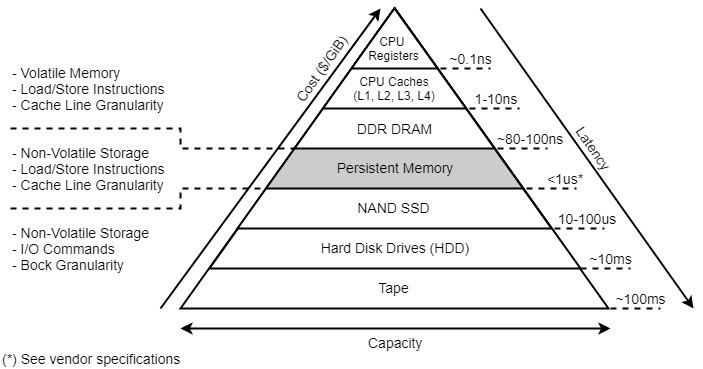
\includegraphics[scale=0.6]{images/pmem_storage_pyramid.jpg}
    \caption{Memory Hierarchy. Taken from \cite{Introduc86:online}}
    \label{fig:pmem_storage_pyramid}
\end{figure}

Persistent memory, also referred to as Non-Volatile Memory (NVM), represents a significant evolution in the memory/storage hierarchy (Figure \ref{fig:pmem_storage_pyramid}), addressing the performance and capacity gap between dynamic random-access memory (DRAM) and traditional storage mediums. This innovative technology combines the characteristics of both DRAM and storage, offering the speed of DRAM and the non-volatile nature of storage devices \cite{scargall2020pmem}.

Like DRAM, persistent memory is available in the form of Dual In-line Memory Modules (DIMMs), which are directly connected to the memory bus. This direct connection enables applications to access persistent memory with the same ease as traditional DRAM, eliminating the need for frequent data transfers between memory and storage. However, unlike DRAM, persistent memory DIMMs provide significantly greater capacity and retain data even when power is removed, thereby enhancing system performance and enabling fundamental changes in computing architecture \cite{rudoff2017persistent,scargall2020pmem}.

Intel Optane DC Persistent Memory Module (Optane PMM) stands at the forefront of commercial implementations of persistent memory technology, leveraging Intel's innovative 3D-XPoint technology. Upon its introduction, the Optane PMM offers substantial capacities up to 512GiB and is exclusively supported by Intel Cascade Lake platform. Each processor within this platform is equipped with two integrated memory controllers (iMCs), with each iMC supporting three channels. This architecture seamlessly integrates Optane PMM with DRAM, allowing users to deploy up to one Optane PMM per channel and up to six per CPU socket, thereby enabling extensive memory capacities of potentially up to 3TiB per socket \cite{yang2020empirical,izraelevitz2019basic}.

Similar to conventional DRAM DIMMs, Optane PMMs are positioned on the memory bus and connect directly to the processor's iMC. The communication protocol between the iMC and the Optane PMM is depicted in Figure \ref{fig:optane_communication}.  Communication between the iMC and the Optane PMM occurs via the DDR-T protocol, adapted for persistent memory and operating at cache line granularity (64B). Initial memory access to the Optane PMM is coordinated by the onboard Controller, which manages access to the 3D-XPoint media. Analogous to SSDs, the Optane PMM conducts address translation for wear-leveling and bad block management, facilitated by the maintenance of an address indirection table (AIT). Following translation, access to the storage media occurs. Notably, with 3D-XPoint access granularity set at 256B, the controller converts 64-byte accesses into 256-byte accesses, inducing write amplification. To mitigate this, the Controller incorporates a 16KB write-combining buffer to merge adjacent writes \cite{yang2020empirical,izraelevitz2019basic,wu2020ribbon}.

\begin{figure}[ht]
    \centering
    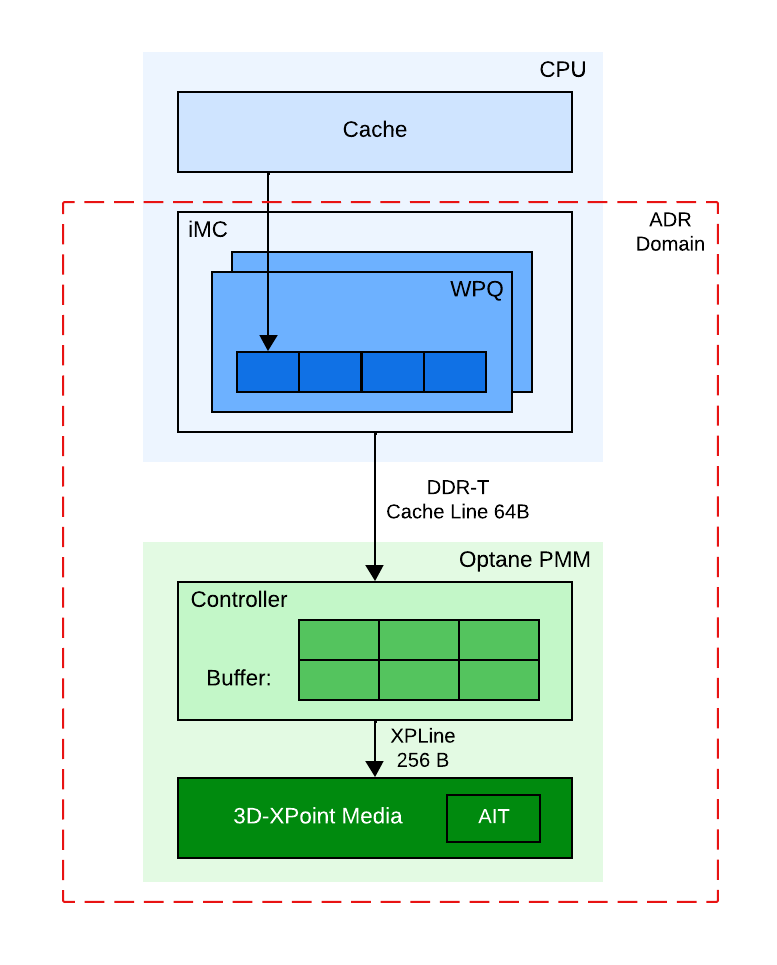
\includegraphics[scale=0.7]{images/optane-communication.png}
    \caption{Communication between iMC and Optane PMM}
    \label{fig:optane_communication}
\end{figure}

To ensure data persistence, Intel platforms integrate the iMC and Optane PMM within the asynchronous DRAM refresh (ADR) domain. Intel's ADR feature ensures that CPU stores that reach the ADR domain will survive a power failures \cite{yang2020empirical}. The iMC manages read and write pending queues for each Optane PMM, with the ADR domain encompassing the write pending queue. Once data reaches the write pending queue, ADR ensures its persistence within Optane PMM in the event of power failures. The ADR domain excludes the CPU caches, necessitating additional steps beyond simply executing a store instruction to ensure data persistence. To achieve this, CPU stores must be continually flushed using specialized instructions provided by Intel's Instruction Set Architecture (ISA), including \textrm{CLFLUSH}, \textrm{CLFLUSHOPT}, and \textrm{CLWB} \cite{yang2020empirical,izraelevitz2019basic,rudoff2017persistent}.

\subsection{Performance Characterization}
Previous studies \cite{yang2020empirical,izraelevitz2019basic} conducted an empirical performance assessment of Optane PMM, revealing its nuanced behavior compared to DRAM. They observed that Optane's performance varies significantly depending on specific access patterns, including access size, type, and concurrency level. Notably, they found that Optane's read latency is three times slower than that of DRAM, primarily due to Optane's longer media latency. However, sequential access patterns demonstrate notably improved latency, indicating Optane PMM's capability to consolidate adjacent requests into single 256-byte accesses. The study also highlights that Optane PMM achieves a maximum random read bandwidth of 6.6 GB/s and a write bandwidth of 2.3 GB/s. Moreover, sequential access further enhances bandwidth performance, exhibiting up to a fourfold increase \cite{yang2020empirical,izraelevitz2019basic}.

An insightful observation highlighted by Izraelevitz et al. \cite{izraelevitz2019basic} is that Optane PMM's bandwidth can become saturated when utilized in real-world multi-threaded applications, thereby introducing performance overhead. This phenomenon arises due to Optane PMM's inability to scale performance proportionally with increased thread count, primarily due to contention occurring within the processor's integrated memory controller (iMC) and Optane PMM's buffer. Contentious conditions within the buffer exacerbate the frequency of evictions and write-backs to the 3D-XPoint media, resulting in Optane writing more data internally than what the application necessitates. Furthermore, given Optane PMM's slightly slower performance compared to DRAM, the slower drainage of write pending queues by Optane PMMs introduces head-of-line blocking effects. As the number of threads concurrently accessing Optane PMM increases, contention on the device escalates, heightening the likelihood of the processor experiencing blocking while awaiting completion of previous store operations \cite{yang2020empirical}.

\subsection{Operating Modes and Applications}

Intel Optane persistent memory (PMem) offers two distinct operating modes: Memory mode and App Direct mode.

In Memory mode, Optane PMem serves as a high-capacity main memory without persistence. In this configuration, DRAM is concealed from users and acts solely as a cache for Optane PMem, seamlessly managed by the operating system \cite{yang2020empirical}. 

Conversely, in App Direct mode, Optane PMMs are directly exposed to the operating system as independent persistent memory devices, thus enabling their utilization for persistent storage \cite{izraelevitz2019basic}. Functionally, the operating system perceives DRAM and Optane PMem as distinct memory pools, with the latter offering data persistence. Applications can access Intel Optane persistent memory through direct load/store operations or via a file system configured with the \textrm{dax} (direct access) option. Such a file system is termed as a PM-aware file system, facilitating direct access to persistent memory without relying on the page cache \cite{rudoff2017persistent}.

In the context of this thesis, Optane PMem is exclusively employed in App Direct Mode, coupled with a PM-aware file system to harness its storage capabilities.

\subsection{Programming Persistent Memory}

In the realm of persistent memory technology, maintaining data consistency across runtime and system reboots is essential. To address this challenge, prior research underscores the necessity for applications leveraging persistent memory to implement transactions that are atomic, consistent, thread-safe, and resilient to system failures—a paradigm akin to ACID transactions in database systems. However, achieving such robustness in real-world scenarios poses significant complexity. Recognizing this, Intel has developed the Persistent Memory Development Kit (PMDK) to tackle this challenge \cite{scargall2020pmem,rudoff2017persistent}.

PMDK comprises a comprehensive suite of libraries and tools tailored for both application developers and system administrators, aiming to streamline the management and utilization of persistent memory devices. Drawing on the SNIA NVM Programming model \cite{NVMProgr73:online} as its foundation, these libraries extend its capabilities to varying extents. Some libraries offer simplified wrappers around operating system primitives, facilitating ease of use, while others provide sophisticated data structures optimized for persistent memory usage \cite{scargall2020pmem}.

In the scope of this thesis, we leverage pmemkv \cite{GitHubpm66:online}, a persistent local key-value store provided by PMDK. Designed with cloud environments in mind, pmemkv complements PMDK's suite of libraries with cloud-native support, abstracting the intricacies of programming with persistent memory through a familiar key-value API. Notably, pmemkv distinguishes itself from traditional key-value databases by enabling direct access to data. This means that reading data from persistent memory circumvents the need for copying it into DRAM—an approach that significantly enhances the performance of applications leveraging persistent memory \cite{scargall2020pmem}.

\section{Serverless Computing}

Serverless computing, a prominent execution model within cloud computing, revolutionizes the deployment process by allowing developers to deploy code without the need for provisioning or managing server infrastructure. Although termed "serverless," this model still utilizes servers provided by cloud vendors to execute developers' code. However, the distinguishing feature lies in the abstraction of infrastructure management from the developer's perspective. Developers no longer concern themselves with resource provisioning, scaling, fault tolerance, monitoring, or security patches; instead, they focus solely on code development. Cloud providers take on the responsibility of handling these infrastructure-related tasks on behalf of their customers. Consequently, developers are charged based on the execution time and resources consumed during their code invocations, offering a pay-per-use billing model \cite{jonas2019cloud,romero2021faat,klimovic2018pocket}.

At the heart of serverless computing lies Function-as-a-Service (FaaS), introduced by AWS Lambda in 2015. Since then, various commercial and open-source alternatives have emerged, including Google Cloud Functions, Azure Functions, Apache OpenWhisk, and others. FaaS enables developers to express application logic as stateless functions written in high-level languages such as Java, Python, C, or C++. These functions are packaged together with their dependencies and submitted to the serverless platform. Additionally, developers associate events with each function, such as HTTP requests, file uploads, database triggers, and more. Upon the occurrence of a trigger, the cloud provider promptly executes the associated function, offering a scalable and event-driven approach to application development and deployment \cite{AWSLambd40:online,AzureFun49:online,CloudFun3:online,ApacheOp28:online}.

\subsection{Storage for FaaS}



\section{Reinforcement Learning}

Reinforcement Learning (RL) is a subfield of machine learning concerned with learning optimal decision-making policies through interactions with an environment \cite{sutton2018reinforcement}. 

\subsection{Overview of Reinforcement Learning}
The fundamental concept underlying RL is the notion of an agent, which takes actions in an environment and receives feedback in the form of rewards, indicating the quality of its decisions. The agent's objective is to learn a policy that maximizes cumulative rewards over time. Moreover, the agent is not provided with explicit instructions on which actions to take; instead, it must discover the actions that lead to the highest rewards by trying them.

\begin{figure}[ht]
    \centering
    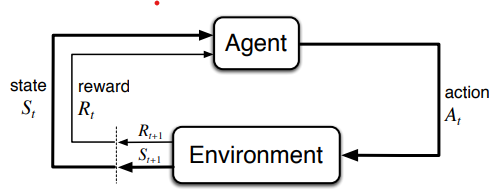
\includegraphics[scale=1]{images/rl-workflow.png}
    \caption{RL Workflow}
    \label{fig:sutton_rl_workflow}
\end{figure}

Figure \ref{fig:sutton_rl_workflow} presents a schematic representation of a standard reinforcement learning scenario. In discrete time steps, the agent perceives the current state $s_t$ from the set of all possible states $S$. It then selects an action $a_t$ from the available actions $A(s_t)$ in the current state. The environment transitions to a new state $s_{t+1}$, and the agent receives a reward $r_t$ associated with the transition $(s_t, a_t, s_{t+1})$.

The agent's behavior is governed by its policy, which maps perceived states to actions. The ultimate aim is to learn an optimal or near-optimal policy that maximizes the cumulative reward. 


\subsection{Q-Learning}

One of the foundational algorithms in RL is Q-Learning, introduced by Watkins in 1989 \cite{watkins1989learning}. The algorithm belongs to the class of model-free RL algorithms, meaning it learns directly from experience without requiring a model of the environment dynamics \cite{russel2020ai}.

At the core of Q-Learning is the Q-value function, denoted as $Q(s, a)$, which represents the expected cumulative reward the agent will receive by taking action $a$ in state $s$ and following an optimal policy thereafter. The objective of Q-Learning is to iteratively update the Q-values based on observed transitions and rewards, eventually converging to the optimal Q-values that maximize long-term rewards.

The Q-Learning algorithm proceeds as follows: the agent interacts with the environment by selecting actions based on its current estimate of the Q-values. Upon taking an action, the agent observes the resulting reward and the next state. It then updates the Q-value of the previous state-action pair using the observed reward and the estimated value of the next state.

The Q-value update rule in Q-Learning is based on the Bellman equation, which expresses the relationship between the Q-values of successive states \cite{russel2020ai}:

\[
Q(s, a) \leftarrow (1 - \alpha) \cdot Q(s, a) + \alpha \cdot \left( r + \gamma \cdot \max_{a'} Q(s', a') \right)
\]

Here, $\alpha$ is the learning rate, determining the extent to which new information overrides the old one, and $\gamma$ is the discount factor, representing the importance of future rewards relative to immediate rewards. The term $r + \gamma \cdot \max_{a'} Q(s', a')$ is known as the temporal-difference (TD) target, combining the immediate reward $r$ with the discounted maximum Q-value of the next state $s'$ \cite{russel2020ai}.

% Q-Learning, a model-free reinforcement learning algorithm, is employed by the agent to determine the best action given the current state. The agent evaluates action quality using a quality-function (Q-function) $Q(s, a)$, representing the expected total discounted reward if the agent selects action $a$ in state $s$ and acts optimally thereafter. 

% One of the foundational algorithms in RL is Q-Learning, introduced by Watkins in 1989 \cite{watkins1989learning}. Q-Learning is a model-free algorithm that learns the value of taking an action in a particular state, known as the Q-value, and iteratively refines these values through experience. The Q-value represents the expected cumulative reward the agent will receive by taking an action in a given state and following an optimal policy thereafter.

% The Q-Learning algorithm (illustrated in Figure \ref{algo:q_learning}) involves iterative updates to the Q-function. At each step, the agent selects an action, observes the reward and new state, and then applies one-step Q-learning. The update is governed by the Q-learning formula, where the learning rate ($\alpha$) determines the extent to which new information overrides old data. This learned Q-function approximates the optimal Q-function, irrespective of the policy being followed.

\subsection{Linear Regression Models in Reinforcement Learning}

One of the key advantages of Q-Learning is its simplicity and ease of implementation. It requires only a table to store the Q-values, making it computationally efficient for small state and action spaces. However, Q-Learning faces challenges in environments with large state spaces, as maintaining a lookup table becomes infeasible due to memory and computational constraints.

Function approximation is a fundamental technique in reinforcement learning (RL) aimed at approximating the Q-Value function when dealing with large state or action spaces where tabular representations become impractical \cite{russel2020ai}. This approach allows RL agents to generalize from observed states to unseen states, facilitating decision-making in unexplored regions of the state space.

In the context of RL, linear regression models are commonly used for function approximation \cite{sutton2018reinforcement}.  These models approximate the Q-value function by leveraging a weighted linear combination of features, with each feature capturing a distinct aspect of the state space. Employing gradient-descent methods, notably stochastic gradient descent, enables iterative refinement of the parameters governing the linear function, aimed at minimizing a predefined loss function. This iterative optimization process empowers the model to progressively enhance its predictive accuracy and capture intricate patterns within the state-action space.

Hyperparameter tuning is a critical aspect of training linear regression models in RL \cite{bergstra2012random}. Hyperparameters, such as the learning rate, regularization strength, and feature scaling, significantly impact the performance and convergence of the models. A systematic approach to hyperparameter tuning involves experimenting with different combinations of hyperparameters, evaluating the performance of the trained models on a validation set, and selecting the optimal hyperparameters based on predefined criteria, such as validation error or performance metrics \cite{russel2020ai}.

\subsection{Exploration-Exploitation Tradeoff}

The exploration-exploitation tradeoff poses a significant challenge in reinforcement learning \cite{sutton2018reinforcement}. The agent must strike a balance between exploring unfamiliar actions to gather information and exploiting known actions for immediate rewards. Finding this balance is crucial for effective learning and task performance, as the agent gradually favors actions with higher expected rewards.

One classic strategy for balancing exploration and exploitation is the epsilon-greedy (e-greedy) algorithm \cite{sutton2018reinforcement}. The e-greedy policy selects the action that maximizes the estimated value with probability $1 - \epsilon$ (exploitation) and selects a random action with probability $\epsilon$ (exploration). This approach ensures that the agent continues to explore the environment while gradually exploiting more rewarding actions as it gains knowledge.

Decayed e-greedy methods aim to strike a balance between exploration and exploitation by gradually reducing the exploration rate $\epsilon$ as the agent gains more experience or as the training progresses \cite{sutton2018reinforcement}. This decay encourages the agent to explore the environment more extensively in the early stages of learning while gradually shifting towards exploitation as it becomes more knowledgeable.

\subsection{Reward shaping}

Reward shaping is a technique in reinforcement learning (RL) aimed at accelerating learning by modifying the reward signal provided to the agent. Traditional RL algorithms rely solely on sparse reward signals, which can make learning slow and inefficient, especially in complex environments. Reward shaping addresses this issue by providing additional, shaped rewards that guide the agent towards desirable behaviors. These shaped rewards are designed to provide more informative feedback to the agent, encouraging it to explore the state-action space more effectively. However, reward shaping must be carefully designed to avoid unintended consequences such as overfitting to the shaped rewards or incentivizing undesirable behaviors \cite{russel2020ai}.


%% include the following commands if there are any appendices
\appendix
\appendixeqnumbering

%% A sample appendix
%%
%%**********************************************************************
%% Legal Notice:
%% This code is offered as-is without any warranty either
%% expressed or implied; without even the implied warranty of
%% MERCHANTABILITY or FITNESS FOR A PARTICULAR PURPOSE!
%% User assumes all risk.
%% In no event shall any contributor to this code be liable for any damages
%% or losses, including, but not limited to, incidental, consequential, or
%% any other damages, resulting from the use or misuse of any information
%% contained here.
%%**********************************************************************
%%
%% $Id: Appendix.tex,v 1.5 2006/08/24 21:12:47 Owner Exp $
%%

% N.B.: an appendix chapter starts with "appchapter" instead of "chapter"
%
% The first argument in [ ] is the title as displayed in the table of contents
% The second argument is the title as displayed here.  Use \\ as appropriate in
%   this title to get desired line breaks
\appchapter[An Appendix]{An Appendix}

This is an appendix.  Here is a numbered appendix equation:
\begin{equation}
    a^2 + b^2 = c^2.
\end{equation}

\newpage
appendix page 2
\begin{equation}
	a^2 + b^2 = c^2.
\end{equation}
\pagebreak
\section{section}
\subsection{subsection}
\subsubsection{subsubsection}



%%
%%  bibliography
%%

%% Use the bibliographicstyle command to use a .bst file for your citation style. If you use biblatex, comment this out and use it as directed in the package documentation.
\bibliographystyle{unsrt}
% The .bib file is gmuETD.bib
\bibliography{gmuETD}

%%
%% biography
%%
\biography

\noindent Include your \emph{biography} here detailing your background, education, and professional experience.
\end{document}
